\chapter{Introduction}
\label{chapter:introducao}

This chapter starts with the context and delimitation of research problem (\autoref{sec:problem-delimitation}). After that, the chapter formulates the research questions and objectives (\autoref{sec:research-question-and-research-objectives}). The research methodology is presented in \autoref{sec:research-methodology}. The thesis statement and contributions are presented in \autoref{sec:thesis-statement-and-claimed-contributions}. The chapter ends with the structure of this dissertation (\autoref{sec:structure-of-dissertation}).

\section{Context and Problem Delimitation}
\label{sec:problem-delimitation}

Over the last two decades or so, with the growing number of technologies that enable people to communicate and work in group activities using computers and Internet, researches and practitioners have developed technology and software applications that facilitate and foster the Collaborative Learning (CL) \cite{LehtinenHakkarainenLipponenRahikainenMuukkonen1999}. Such technology and the research field that studies how to effectively link together the advanced in computer science with the collaborative learning is known as Computer-Supported Collaborative Learning (CSCL), and it has been proved an important to support the learning process of students by cognitive, social and technological reasons \cite{StahlKoschmannSuthers2006}. However, CSCL is only beneficial when there is an adequate design establishing the way in which the collaboration should happened \cite{Dillenbourg2013, Hewitt2005, IsotaniInabaIkedaMizoguchi2009}. Students frequently fail to be engaged in productive learning interactions when they are left to interact in CL activities without any support. Hence, several researchers propose the use of scripts to guide and orchestrate the collaboration among students \cite{AlharbiAthaudaChiong2014}.

Scripted collaboration aims to engage the students in fruitful and meaningful interactions according to a design that has the purpose to attain a set of pedagogical objectives. Thereby, CSCL scripts have been proposed by the community to support the well-thought-out design of the CL scenarios by means of computer-based systems \cite{FischerKollarStegmannWeckerZottmann2013,KobbeWeinbergerDillenbourgHarrerHamalainenHakkinenFischer2007}. These scripts are the technology that describes how the interactions among students will be orchestrated in a group activity to increase the possibility of achieving the pedagogical objectives \cite{WeinbergerErtlFischerMandl2005}. These scripts provide information that facilitates the group formation, the role distribution, and the sequencing of interaction for the participants of a CL activity. Despite of these benefits, there are situations in which the scripts may cause motivational problems. For example, when a student prefers to work individually, or when he/she does not want to play the role assigned by the scripts, the student may neglect his/her personal behavior to get the task completed without effort, and the lack of choice over the sequence of interactions may produce in the student a sense of obligation in complete an unwilling activity.
These issues negatively influence the student's motivation, learning attitudes and behaviors, so that the group dynamic is degraded resulting in negative and widespread learning outcomes.

The motivational problems caused by the scripted collaboration makes more difficult the use of CSCL technology over time. In fact, less motivated students prefer to spend more time in other activities rather than to learn and, as consequence, the achievement of expected learning outcomes becomes difficult \cite{Crook2000, FaloutElwoodHood2009, SchoorBannert2011}. In this sense, motivating learners in the entire instructional process of CL is important. However, the traditional instructional design practice often assumes that the motivation is a simple preliminary step that must happen before the instruction \cite{ChanAhern1999, Keller1987}. This assumption is based in which the good quality of learning materials can keep the students focused during the learning process, but if this process is long, there is a good chance that the students will lose their initial motivation. To solve this problem, several approaches, such as the use of affective feedbacks based on emotion-aware systems \cite{FeidakisDaradoumisCaballeConesa2014,FeidakisCaballeDaradoumisJimenezConesa2014}, and learning companions \cite{WoolfBurlesonArroyoDragonCooperPicard2009}, and so on, have been proposed to motivated students along the entire learning process. These solutions assume that the students like the content-domain and/or have the desired to learn, so that students that do not have the desire to learn are not motivated and engage for these approaches.

In the last years, efforts of CSCL community have been directed to finding new innovative solutions that, beside to motivate and engage students during the entire CL process, are not completely tied to the domain-content and desired to learn the domain-content.
In this direction, several researchers and practitioners have pointed Gamification as a promising technology to deal with motivational problems in the instructional/learning domain \cite{ChallcoMoreiraMizoguchiIsotani2014, SeabornFels2015, BorgesDurelliReisIsotani2014}.
Gamification defined \aspas{\emph{as the use of game design elements in non-game contexts}} \cite{DeterdingDixonKhaledNacke2011} aims to increase the students' motivation and engagement by making the learning process more game-like. This is done through the introduction of game elements, such as points, leaderboards, competition, cooperation and so on. These elements are not part of the domain-content, neither they belong to the instructional/learning process, so that they can even motivate students who do not have the desire and/or interest in to learn the content-domain. These game elements are introduced along the entire learning process, so that the benefits of gamification strongly depend on how well these game elements are applied, and how well they are linked with the pedagogical approaches \cite{Kapp2012, KnutasIkonenNikulaPorras2014}.

When CL scenarios are gamified to deal with the motivational problems caused by the scripted collaboration, the author of this thesis hypothesizes that the chances to achieve engagement and educational benefits will be increased whether there is a proper connection between the game elements and the CL process. Nevertheless, developing such well-though-out gamified CL scenario, hereinafter referred to as gamified CL scenarios, is not trivial. The main difficulty to gamify CL scenarios as well as other non-game context is that the gamification is too context dependent \cite{HamariKoivistoSarsa2014, RichardsThompsonGraham2014}. Its effects vary individual to individual, and they depend of many factors such as the individual personality traits, preferences, and current student's emotions \cite{Nicholson2015, PedroLopesPratesVassilevaIsotani2015} (e.g., a user who likes competition would be more motivated by a leaderboard rather than a user who want to obtain items to customize his/her avatar). Also, the expected effects of the game elements vary according to the non-game context and target behavior that is being gamified \cite{DeterdingBjorkNackeDixonLawley2013, HeeterLeeMedlerMagerko2011} (e.g., gamifying a learning scenario to promote the sign-up of participants is not the same that gamifying an interactive environment to maintain the students attention). As consequence of this context-dependency, when a CL scenario is not well gamified, instead to have a positive effect, they may cause a detrimental on the students’ motivation \cite{AndradeMizoguchiIsotani2016}, cheating \cite{NunesBittencourtIsotaniJaques2016}, embarrassment \cite{OhnoYamasakiTokiwa2013}, and lack of credibility on badges \cite{DavisSingh2015}.

Another difficulty to gamify CL scenarios, as well as other non-game contexts, it is the lack of approaches to systematically represent, in an unambiguous way, the gamification knowledge acquired in the last years by researchers and practitioners. This knowledge constituted by theories and practices related to gamification lacks of a formal and common vocabulary, definitions, and representation to apply gamification. As can be appreciated in the current literature of gamification \cite{DichevaDichevAgreAngelova2015, HamariKoivistoSarsa2014, MoraRieraGonzalezArnedo-Moreno2015, SeabornFels2015}, each author proposes his/her own definitions, classifications and representation to describe the concepts and characteristics about how to gamify a non-game context. This fact hinders the creation of models and/or frameworks that formally represent the gamification and its application by computer-based systems in a common understandable and sharable manner, and to the best of the thesis author’s knowledge, there are no one approaches has been proposed to represent the knowledge about how to gamify CL scenarios to deal with motivational problems caused by the scripted collaboration.

Due to the variety of students who can participate in CL sessions, the diversity of subjects that can be under study in a CL activity, and the range of different CSCL scripts that can be used to orchestrate the CL process, it is necessary to personalize the gamification, providing a tailored gamified CL scenario for each situation. This task is difficult and time-consuming, so that developing a computational based-support in intelligent-theory aware systems to give assistance with the personalization of gamification is very helpful and necessary. In this direction, in the context of CSCL, one interesting solution has been proposed to gamify CL scenarios using adaptive profiles and machine learning techniques \cite{KnutasIkonenMaggioriniRipamontiPorras2014,KnutasIkonenNikulaPorras2014}. However, this solution is not oriented to deal with motivational problems caused by the scripted collaboration, its purpose is to increase the communication among the participants in CL scenarios. Furthermore, this solution falls into the category of computer-based mechanisms and procedures that support the gamification, it does not provide a model to share the theoretical knowledge related to gamification obtained by this computer-based mechanism. Solutions based on machine learning to personalize gamification require a lot of data to support the personalization of gamification, and they may have overfitting or underfitting problem with the data. A computer mechanism based only in machine learning techniques to personalize gamification lacks of theoretical-justification to explain why a game element is introduced, and why a certain configuration of game elements increases the motivation participants in a CL scenario.

For the reason exposed above, to deal with motivational problems caused by the scripted collaboration through the gamification of CL scenarios, a computational support with a common and shareable structure to describe knowledge extracted from the practices and theories related to gamification is essential to overcome the challenges and difficulties of gamification. In the direction to make explicit the knowledge contained in computer-based mechanisms and procedures, ontologies have been consolidated as the most advanced technology to support the representation of knowledge in a common computer-understandable and sharable manner \cite{AsikriLaassiriKritChaib2016, Devedzic2006, MizoguchiBourdeau2016}. Ontologies constitute an explicit mapping between the target world of interest and its representation with the purpose to describe concepts without ambiguities providing a common way to represent the knowledge \cite{GuarinoOberleStaab2009}. Taking advantages of this commonality, and using the computer interconnection technologies such as Internet, computer-based mechanisms in intelligent systems use ontologies to share understandings and interpretations of target world. In this direction, employing ontologies, some interesting and practical results have been obtained in the formalization and organization of knowledge extracted from different theories and practices related to gamification \cite{DermevalVilelaBittencourtCastroIsotaniBritoSilva2016, KarkarAlJa'amFoufou2016, ZouaqNkambou2010}. However, currently, there is no one ontology that allows the description of fundamentals concepts extracted from the practices and theories related to gamification, and how these concepts are applied in CL scenarios to deal with the motivational problems caused by the scripted collaboration.

Therefore, the general research goal in this PhD thesis dissertation refers to the definition of an ontology to, from a philosophical perspective, systematically formalize the knowledge extracted from the practices and theories related to gamification, and the definition of computer-based mechanisms that employ this ontology to deal with motivational problem caused by the scripted collaboration in CL activities where the CSCL scripts are used as a method to orchestrate and structure the collaboration among students.

\section{Research Questions and Research Objectives}
\label{sec:research-question-and-research-objectives}

The overarching research question (\textbf{RQ}) answered in this PhD thesis dissertation is: \aspas{\emph{How can gamification and ontologies be used to deal with motivational problems caused by the scripted collaboration in CL activities where CSCL scripts are used as a method to orchestrate and structure the collaboration among students?}}

To answer this research question, the author of this thesis proposes the ontological engineering approach to gamify CL scenarios shown in \autoref{fig:ontological-engineering-approach-to-gamify-cl-scenarios}. This approach consists into three major stages described as follows:

\begin{figure}[htb]
 \caption{Ontological engineering approach to gamify CL scenarios}
 \label{fig:ontological-engineering-approach-to-gamify-cl-scenarios}
 \centering
 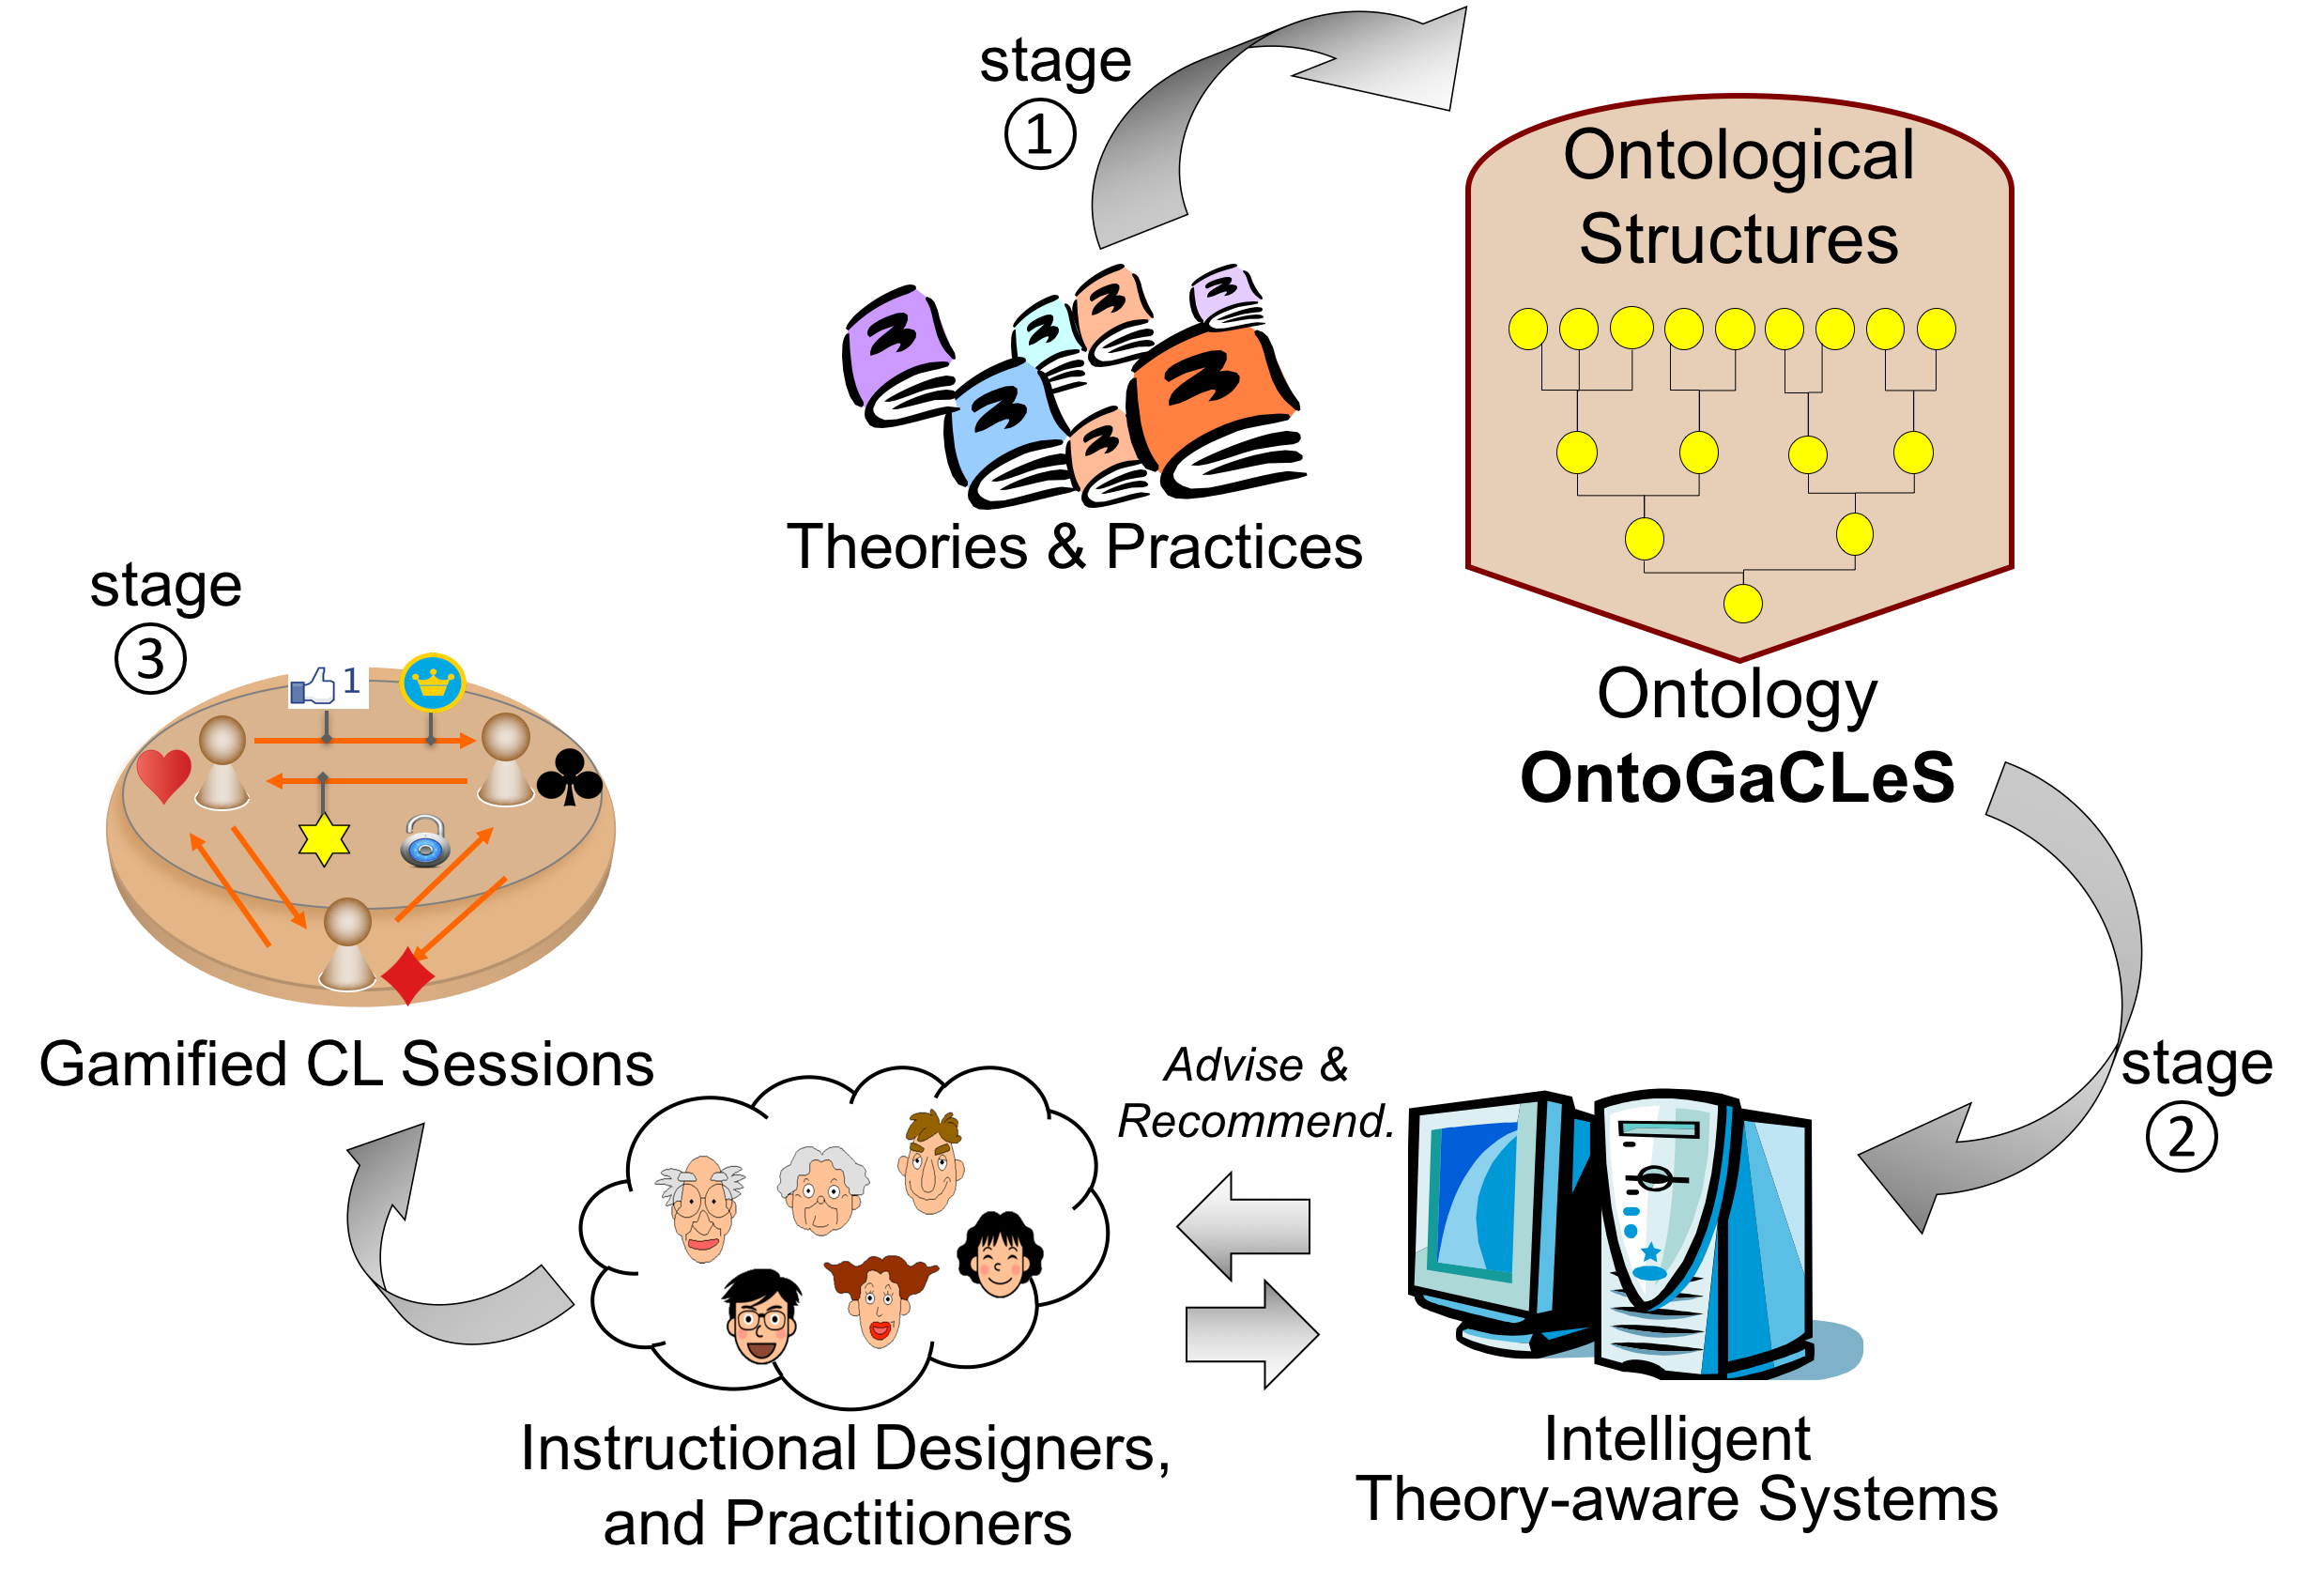
\includegraphics[width=0.9\textwidth]{images/chap-introduction/ontological-engineering-approach-to-gamify-cl-scenarios.png}
 \fautor
\end{figure}

\begin{enumerate}
\item
The first stage is the formalization of the necessary knowledge about how to gamify CL scenarios for dealing with the motivational problems caused by the scripted collaboration into an ontology named \textbf{OntoGaCLeS} – \emph{\textbf{Onto}logy to \textbf{Ga}mify \textbf{C}ollaborative \textbf{Le}arning \textbf{S}cenarios}. This ontology has been developed using ontology engineering in which, by extracting concepts from the theories and practices related to gamification, the author of this thesis defines a set of ontological structures that enables the systematic formalization and representation of necessary knowledge to gamify CL scenarios.

\item
The second stage is the development of computer-based mechanisms and procedures whereby intelligent theory-aware systems will provide support in the gamification of CL scenarios to deal with motivational problems caused by the scripting collaboration. Such support is given by the knowledge formalized in the ontology OntoGaCLeS during the first stage, and the purpose of the computer-based mechanisms is to use this knowledge to facilitate the tasks of instructional designer and practitioners, especially novice users, in the gamification of CL scenarios. This knowledge provides theoretical justification for the personalization of gamification and, thus, to obtain tailored gamified CL sessions adapted for each situation. Such sessions are known as ontology-based CL sessions, and they are CL scenarios that have been gamified and instantiated at the most concrete level by detailing the participants and content-domain to be directly run in a learning environment.

\item
The third stage is the validation of the ontological engineering approach to gamify CL scenarios as a method to deal with motivational problems caused by the scripted collaboration. This validation is carried out in ontology-based gamified CL sessions obtained by the approach, and it consists in measuring the effectiveness and efficiency of these sessions for dealing with motivational problems caused by the scripted collaboration. The effectiveness and efficiency were measured by comparing the effects on students' motivation and learning outcomes caused by ontology-based CL sessions, non-gamified CL sessions and CL sessions gamified without using the support given by the ontology OntoGaCLeS.
\end{enumerate}

Regarding to the formalization of knowledge about how to gamify CL scenarios for dealing with motivational problems caused by the scripted collaboration (Stage 1), the research questions answered by this dissertation are:

\begin{description}
\item[RQ1:]
Which concepts from the theories and practices related to gamification should be taking into account to deal with motivational problems caused by the scripted collaboration? and How should these concepts be applied in the gamification of CL scenarios?

\item[RQ2:]
How can the concepts extracted from the theories and practices related to gamification, and identified as relevant to deal with motivational problems caused by the scripted collaboration, be represented as ontological structures?
\end{description}

Regarding to the development of computer-based mechanisms and procedures whereby intelligent theory-aware systems will provide support in the gamified CL scenarios using the knowledge described in the ontology OntoGaCLeS (Stage 2), the research questions answered by this dissertation are:

\begin{description}
\item[RQ3:]
What computer-based mechanisms and procedure are necessary in intelligent-theory aware systems to give a helpful support in the gamification of CL scenarios? and How can the knowledge encoded in the ontology OntoGaCLeS be used by these mechanisms and procedures for dealing with motivational problems caused by the scripted collaboration?
\end{description}

Regarding to the validation of the ontological engineering approach to gamify CL scenarios as a method to deal with the motivational problems caused by the scripted collaboration (Stage 3), the research questions answered by this dissertation are:

\begin{description}
\item[RQ4:]
What are the effects of ontology-based gamified CL sessions on the students’ motivation and learning outcomes? and What are the effectiveness and efficiency of these sessions to deal with motivational problems caused by the scripted collaboration?
\end{description}

The research objectives pursued to answer the research questions \emph{RQ1} and \emph{RQ2} are:

\begin{description}
\item[RO1:]
To review the scientific literature in order to identify the most relevant concepts from the theories and practices related to gamification that should be taking into account to deal with motivational problems caused by the scripted collaboration, and how these concepts be applied in the gamification of CL scenarios; and

\item[RO2:]
To define the necessary ontological structures to represent the concepts identified as relevant in the scientific literature of gamification to deal with motivational problems caused by the scripted collaboration.
\end{description}


In order to answer the research question \emph{RQ3}, the research objectives is:

\begin{description}
\item[RO3:]
To identify and define the computer-based mechanisms and procedures that must be implemented by intelligent-theory aware systems to give a helpful support in the gamification of CL scenarios, and how these mechanisms and procedure use the knowledge encoded in the ontology OntoGaCLeS for dealing with the motivational problems caused by the scripted collaboration.
\end{description}

The research objective pursued to answer the research question \emph{RQ4} is:

\begin{description}
\item[RO4:]
to analyze the effects of ontology-based gamified CL sessions on the students’ motivation and learning outcomes for the purpose of validating the ontology engineering approach to gamify CL scenarios in reference to the effectiveness and efficiency to deal with the motivational problems caused by the scripted collaboration.
\end{description}

It is out of scope in this dissertation to deal with the following objectives:

\begin{itemize}
\item
To compare, validate or judge the practices and theories related to gamification.

\item
To create, modify or extend the concepts described in the practices and theories related to gamification.

\item
To create a generic and complete representation of all concepts described in the practices and theories related to gamification. The author of this thesis only concentrates on the formalization of the minimal necessary concepts from these practices and theories to deal with the motivational problems caused by the scripted collaboration.

\item
To validate the concepts and ontological structures formalized in the ontology OntoGaCLeS using semantic reasoner engines or formal methods based on logic and/or mathematics.
\end{itemize}

\section{Research Methodology}
\label{sec:research-methodology}

As this PhD thesis dissertation is framed in the multidisciplinary field of CSCL with research questions and research objectives oriented to be answered and achieved by theoretical and empirical studies, a mixed research method needs to be employed to conduct this research. Following the research methodology framework proposed by \citeonline{Glass1995,GlassVesseyRamesh2002}, the mixed research method employed in this PhD thesis research consists in four iterative phases: informational, propositional, analytical and evaluation.

\begin{description}
\item[Informational phase:]
In this phase, the research problems and potential solutions were identified based on information gathered from the scientific literature and discussions with experts in fields of CSCL, gamification and ontology engineering. The results of this phase were an outline of the knowledge involved in this dissertation, the research questions, and the research objectives. The tasks carried out in this phase correspond to tasks extracted from the scientific (observing the world) and engineering (observing existing solutions) research methods. These tasks were:

\begin{itemize}
\item
The search, review and analysis of scientific literature regarding to: CSCL, gamification and ontology engineering. This literature review was performed with emphasis in scripted collaboration, gamification of learning and instruction, and ontology-engineering applied to Artificial Intelligence in Education (AIED).

\item
The participation as member of the research group in Applied Computing in Education Laboratory (CAEd-Lab, \emph{Laboratorio de Computação Applicada a Educação e Tecnologias Sociales Avançadas}) at the University of São Paulo. Particularly, the expertise field in CSCL and Ontologies of this research group has been very important and valuable to conduct the research and the literature reviews.

\item
The participation in several conferences and workshops related to the context and problem domain in which this dissertation is framed. These conferences and workshop, in chronological order, were: the III Escola de Ontologias UFAL-USP, 2014 (Workshop); the 20\textsuperscript{th} International Conference on Collaboration and Technology, CRIWG, 2014 (Conference), the Summer School on Computers in Education, 2015 (Workshop); the XXVI Brazilian Symposium on Computers in Education, 2015 (Conference); the 6\textsuperscript{th} Latin American School for Education, Cognitive and Neural Sciences, 2016 (Workshop); and the Higher Education for All: International Workshop on Social, Semantic, Adaptive and Gamification techniques and technologies for Distance Learning, 2017 (Workshop).

\item
The participation as visiting research at the Research Center for Service Science at the School of Knowledge Science in the Japan Advanced Institute of Science and Technology (JAIST) has also been significant for the informational phase. This research center is dedicated to study, design and implementation knowledge co-creation process in complex service systems.  This research center focuses in the use of ontologies and ontology-engineering as the technology to develop and solve a broad variety of domains/tasks, and their research members have a long history working in the research field of Artificial Intelligence in Education. Particularly, the expertise of the Prof. Mitsuro Ikeda and Prof. Riichiro Mizoguchi were valuable and important for this phase due to their involvement in various research projects related to the modeling of knowledge for the students’ learning growth, CL process, and instructional design.
\end{itemize}

\item[Propositional phase:]
In this phase, solutions were proposed and formulated using the information gathered in the previous phase. As results of the propositional phase, constructors of necessary concepts to gamify CL scenarios were identified and proposed as ontological structures in the ontology OntoGaCLeS. Prototypes of computer-based mechanisms and procedures were also developed for gathering practitioner and user opinions as early feedback of these systems. The tasks carried out in this phase correspond to task extracted from the scientific (proposing theories or models) and engineering (proposing and developing solutions) research methods. These tasks were:

\begin{itemize}
\item
The proposal of ontological structures in the ontology OntoGaCLeS to represent gamified CL scenarios and ontological models to personalize the gamification of CL scenarios based on player type models and need-based theories of motivation.

\item
The proposal of ontological structures in the ontology OntoGaCLeS to represent the application of persuasive game design models in gamified CL scenarios and ontological models to apply persuasive game strategies as a method for dealing with the motivational problems caused by the scripted collaboration.

\item
The proposal of a computer-based model to unify the modeling of the learners' growth process and the flow theory based on the principle of good balance between the perceived challenges and skills.


\item
The definition of a conceptual flow to gamify CL scenarios as a computer-based procedure to use the knowledge described in the ontology OntoGaCLeS, and the definition of a reference architecture based on this flow to build computer-based mechanisms that provide support in intelligent-theory aware systems for dealing with the motivational problems caused by the scripted collaboration.
\end{itemize}

\item[Analytical phase:]
This phase consists into analyze and explore the solutions formulated in the propositional phase with the purpose to identify whether the proposed solutions are understandable, how them can be deployed into practice, what are the potential problems in understanding and using them, and wether there are any omissions or gaps in these solutions. The tasks carried out in this phase correspond to task extracted from the empirical (applying to case studies) and analytical (developing new solutions derived from the results obtained in the case studies) research methods. These tasks were:

\begin{itemize}
\item
The formalization of an ontological model to personalize the gamification of CL scenarios based on the Dodecad player type model proposed by \citeonline{Marczewski2015b}, and the formalization of an ontological model to personalize the gamification of Cognitive Apprentice CL scenarios based on the Yee's player type model. These two formalizations were developed as case studies to validate in the evaluation phase the ontological structures proposed to systematically formalize ontological models to personalize the gamification of CL scenarios.

\item
The formalization of an ontological model to apply gamification as a persuasive technology in gamified Cognitive Apprenticeship scenarios employing the persuasive game design strategies defined in the Model-driven persuasive game proposed by \citeonline{Orji2014}.

\item
The implementation of a computer-based mechanism (as a proof of concept) in which the knowledge encoding in the ontology OntoGaCLeS is used for setting up the proper player roles and game elements for CL sessions.

\item
The development of an algorithm (as a proof of concept) to apply the principle of good balance between the perceived challenges and skills from the flow theory in the gamification of CL scenarios.

\item
The development of a computer-based mechanisms (as a proof of concept) to apply gamification as persuasive technology in the gamification of CL scenarios. 
\end{itemize}


\item[Evaluation phase:]
The focus of this phase is to conduct empirical tests and evaluations for the solutions formulated in the propositional phase and for the findings found in the analytical phase. In this phase, the empirical data gathered through the tests and evaluations aim to assess the contributions from different perspectives. The task carried out in this phase correspond to task from the empirical (validating the solutions) and analytical (analyzing the results obtained from empirical observations) research methods. These tasks were:

\begin{itemize}
\item
The analytical evaluation of the ontological structures proposed to represent gamified CL scenarios and the ontological models to personalize the gamification of CL scenarios. This evaluation was carried out by publishing these ontological structures and the ontological models obtained from them in the analytical phase (the ontological model to personalize gamification in CL scenarios based on the Dodecad player type model, and the ontological model to personalize gamification in Cognitive Apprentice CL scenarios based on the Yee's player type model) as scientific articles in conferences and journals related to the fields of CSCL, and Artificial Intelligent in Education. These articles, in chronological order, were: \aspas{\emph{Towards an Ontology for Gamifying Collaborative Learning Scenarios}} published in the 12\textsuperscript{th} International Conference on Intelligent Tutoring Systems, ITS, 2014; \aspas{\emph{An Ontology Engineering Approach to Gamify Collaborative Learning Scenarios}} published in the 20\textsuperscript{th} International Conference on Collaboration and Technology, CRIWG, 2014; and \aspas{\emph{Personalization of Gamification in Collaborative Learning Contexts using Ontologies}} published in the journal of IEEE Latin America Transactions, 2015. During the conferences important feedbacks to improve the ontological structures were obtained from informal discussions with the participants of the conferences who shared their expertise in the domain of CSCL and Artificial Intelligent in Education.

\item
The analytical evaluation of the ontological structures proposed to represent the application of persuasive game design models in gamified CL scenarios and the ontological models to apply persuasive game strategies as a method for dealing with motivational problems caused by the scripted collaboration. This evaluation was carried out by publishing these ontological structures and the ontological models obtained from them in the analytical phase (the ontological model to apply gamification as a persuasive technology in gamified Cognitive Apprenticeship scenarios employing the persuasive game design strategies defined in the Model-driven persuasive game) as scientific articles scientific articles in conferences and journals related to the fields of CSCL, and Artificial Intelligent in Education. These articles, in chronological order, were: \aspas{\emph{Steps Towards the Gamification of Collaborative Learning Scenarios Supported by Ontologies}} published in the 17\textsuperscript{th} International Conference on Artificial Intelligence in Education, AIED, 2015; \aspas{\emph{An Ontological Model to Apply Gamification as Persuasive Technology in Collaborative Learning Scenarios}} published in the 26\textsuperscript{th} Brazilian Symposium of Informatics in Education, SBIE, 2015; \aspas{\emph{Gamification of Collaborative Learning Scenarios: Structuring Persuasive Strategies Using Game Elements and Ontologies}} published in the 1\textsuperscript{st} International Workshop of Social Computing in Digital Education, SOCIALEDU, 2015; and \aspas{\emph{An Ontology Framework to Apply Gamification in CSCL Scenarios as Persuasive Technology}} published in the Brazilian Journal of Computers in Education, 2016. During the conferences important feedbacks to improve the ontological structures were obtained from informal discussions with the participants of the conferences who shared their expertise in the domain of CSCL and Artificial Intelligent in Education.

\item
The conduction of a pilot empirical study in which, prior to carry out the full-scale empirical studies, the activities, methods, instruments and activities that have been used in the full-scale studies were evaluated to adjust and improve the full-scale study design. This empirical study has been conducted to assess the effectiveness of \emph{the ontological engineering approach to gamify CL scenarios} for dealing with the motivational problems caused by the scripted collaboration. Such effectiveness is measured by comparing the effect of the ontology-based CL sessions obtained by the approach against the effect of non-gamified CL sessions on the participants' intrinsic motivation and learning outcomes, and the percentage of participation by groups. This empirical study was conducted with undergraduate computer science students at the university of São Paulo during the second semester of 2016 in the course of Laboratory of Introduction to Computer Science, and for a CL activity related to the topic of loop structures. In such CL activity, the ontology-based gamified sessions and non-gamified CL sessions have been instantiated using a CSCL script inspired by the cognitive apprenticeship theory as the method to orchestrate and structure the collaboration among the students.

\item
The conduction of a full-scale empirical to evaluate the effectiveness of \emph{the ontological engineering approach to gamify CL scenarios}. This effectiveness has been measured by comparing the effects of ontology-based gamified CL sessions against the effects of non-gamified CL sessions on the participants' intrinsic motivation and learning outcomes. This study was carried out in the course of introduction to computer science with undergraduate computer engineering students at the university of São Paulo during the first semester of 2017. The CL activity in which these CL sessions have been instantiated was related to the topic of condition structures using a CSCL script based on the cognitive apprentice theory to orchestrate and structure the collaboration among the participants.

\item
The conduction of a full-scale empirical study to also evaluate the effectiveness of \emph{the ontological engineering approach to gamify CL scenarios}. However, in this empirical study, the effects of ontology-based gamified CL sessions against the effect of non-gamified CL sessions were compared on the participants' level of motivation instead to compare these effects on the participants' intrinsic motivation. This empirical study was carried out during the first semester of 2017 in the course of Introduction to Computer Science at the university of São Paulo with undergraduate computer engineering students. In this context, a CSCL script inspired by the cognitive apprentice theory was used to structure and orchestrate the collaboration among the students a CL activity related to the the topic of loop structures.

\item
The conduction of a full-scale empirical study to evaluate the efficiency of \emph{the ontological engineering approach to gamify CL scenarios} for dealing with the motivational problems caused by the scripted collaboration. Such efficiency was measured by comparing the effects on the participants intrinsic motivation, level of motivation, and learning outcomes caused by ontology-based CL sessions against the effects caused by CL sessions that have been gamified without using the support given by the ontology OntoGaCLeS. This empirical study was carried out in the course of Introduction to Computer Science at the university of São Paulo during the first semester of 2017. The undergraduate computer engineering students signed up in this course participated in a CL activity related to the topic of recursion in which the collaboration among the students was orchestrated and structured by a CSCL script inspired by the cognitive apprentice theory.
\end{itemize}
\end{description}

\section{Thesis Statement and Claimed Contributions}
\label{sec:thesis-statement-and-claimed-contributions}

The thesis statement of this PhD thesis dissertation is that:

\aspas{\emph{For CL activities where the CSCL scripts are used as a method to orchestrate and structure the collaboration among the participants, the gamification of CL scenarios using the support given by the ontology OntoGaCLeS constitutes an effective and efficient solution to deal with the motivational problems caused by the scripted collaboration because this ontology encodes the necessary theoretical knowledge related to theories and practices of gamification to perform this task}.}

The claimed contributions are:

\begin{enumerate}
\item 
The identification of most relevant concepts from the theories and practices related to gamification that should be taking into account to deal with the motivational problems caused by the scripted collaboration (RO1).

\item
Ontological structures that represent the concepts identified as relevant in the theories and practices related to gamification for dealing with the motivational problems caused by the scripted collaboration (RO2).

\begin{enumerate}
\item
A set of ontological structures to represent gamified CL scenarios and ontological models to personalize the gamification of CL scenarios based on player types models and need-based theories of motivation.

\item
A set of ontological structures to apply persuasive game design models in gamified CL scenarios and ontological models to apply persuasive game strategies as a method for dealing with the motivational problems caused by the scripted collaboration.

\item 
A unify modeling of learners' growth process and flow theory as a computer-based model to apply the principle of good balance between the perceived challenges and skills for gamified CL scenarios.
\end{enumerate}

\item
A conceptual flow to gamify CL scenarios using the knowledge described in the ontology OntoGaCLeS, and a reference architecture based on this flow to build computer-based mechanisms that provide support in intelligent-theory aware systems for dealing with the motivational problems caused by the scripted collaboration (RO3).

\item
An empirical evaluation of \emph{the ontological engineering approach to gamify CL scenarios} in which, to validate the effectiveness and efficiency of this approach for dealing with the motivational problems caused by the scripted collaboration, the effects of ontology-based gamified CL sessions on students' intrinsic motivation, level of motivation and learning outcomes are compared against the effects caused by the non-gamified CL sessions and CL sessions that have been gamified without using the support given by the ontology OntoGaCLeS (RO4).
\end{enumerate}

\section{Structure of the Dissertation}
\label{sec:structure-of-dissertation}

This PhD thesis dissertation is structured in eight chapters:

\begin{description}

\item[Chapter 1:]
\emph{Introduction}

\item[Chapter 2:]
\emph{General Background and Fundamental Concepts}
contains the background related to the context and research problem addressed in this dissertation. An overview related to the fields of CSCL and scripted collaboration, gamification and ontology engineering are presented in the chapter. The motivational problems caused by the scripted collaboration, and the current approaches to deal with this problem are also detailed in the chapter. The concepts that were identified as relevant in the theories and practices of gamification and their difficulties to apply it in CL scenarios for dealing with the motivational problems caused by the scripted collaboration are presented in the chapter.

\item[Chapter 3:]
\emph{Ontological Structure to Personalize the Gamification in CL Scenarios} describes the ontological structures, that have been proposed by the author of this thesis, and that have been formalized in the ontology OntoGaCLeS, to represent gamified CL scenarios and ontological models to personalize the gamification in CL scenarios based on player types models and need-based theories of motivation. The chapter also shows the procedure followed to build an ontological model ontological model to personalize the gamification of CL scenarios based on the Dodecad player type model. 

\item[Chapter 4:]
\emph{Ontological Structures of Persuasive Game Design in CL Scenarios} describes the ontological structures proposed by the author of this thesis to apply persuasive game design models in gamified CL scenarios and to represent ontological models to apply persuasive game strategies as a method for dealing with the motivational problems caused by the scripted collaboration. The chapter also describes the procedure to formalize an ontological model in which gamification is applied as persuasive technology for gamified Cognitive Apprenticeship scenarios employing the persuasive game design strategies defined in the Model-driven persuasive game proposed by \citeonline{Orji2014}.

\item[Chapter 5:]
\emph{A Unify Modeling of Learners' Growth Process and Flow Theory} presents the computer-based model proposed by the author of this thesis to unify the modeling of the learners' growth process and the flow theory based on the principle of good balance between the perceived challenges and skills. This model has been used in the gamification of CL scenarios to define the rewards to be promised and given to maintain the learner's flow state in the CL process.

\item[Chapter 6:]
\emph{Computer-based Mechanisms and Procedures to Gamify CL Scenarios} describes the flow proposed by the author of this thesis to use the knowledge described in the ontology OntoGaCLeS to gamify CL sessions. The reference architecture based on this flow by which computer-based mechanisms could be built in intelligent-theory aware systems to provide support in the gamification of CL scenarios for dealing with the motivational problems caused by the scripted collaboration is presented in the chapter. The chapter also describes the computer-based mechanisms that has been developed by the author of this thesis using the reference architecture to conduct the evaluation of the ontological engineering approach to gamify CL scenarios.

\item[Chapter 7:]
\emph{Evaluation of the Ontological Engineering Approach to Gamify CL Scenarios} presents the empirical studies that have been carried out in real situations to validate the effectiveness and efficiency of this approach to deal with the motivational problems caused by the scripted collaboration.

\item[Chapter 8:]
\emph{Conclusions and Future Work} summarizes the contributions of this PhD thesis dissertation, and the chapter also discusses possible future research directions.

\end{description}




